\documentclass{fefu}

\usepackage{graphicx}
\usepackage{float}
\usepackage{wrapfig}

\begin{document}
	\setschool{ШКОЛА ЕСТЕСТВЕННЫХ НАУК}
	\setdepartment{кафедра информатики, математического и компьютерного 
	моделирования}{А.Ю.Чеботарев}
	\setgroup{Б8403а}
	\title{о прохождении преддипломной практики\\направление подготовки 01.03.02 
	Прикладная математика и информатика\\профиль «Системное программирование»}
	\setdates{29}{апреля}{2019}{22}{июня}{2019}
	\setweeks{8}
	\setplace{кафедре информатики, \\математического и компьютерного \\моделирования}
	\author{Куцелабский Е.С.}
	\setsupervisor{Петров П.С.}
	
	\makereporttitle
	\tableofcontents
	\newpage
	
	\begin{abstract}
		\par Текущая версия текстового редактора в open-source движке Citrus малоэффективна.
		Целью данной работы является разработка нового текстового редактора для 
		движка. В работе изложены особенности реализации и принятые решения.
		Выполнено сравнение производительности между предыдущей версией редактора и
		новой реализацией.
	\end{abstract}

	\section{Введение}
		\subsection{Глоссарий}
			\begin{itemize}
				\item Текстовый редактор ---
				\item Игровой движок --- 
				\item Сборка проекта ---
				\item Компоновка библиотек ---
				\item Сериализация ---
				\item Частота кадров ---
				\item Алгоритмическая сложность ---
			\end{itemize}
		\subsection{Описание предметной области}
			\subsubsection{Студия Game Forest}
				\par Заказчиком данной работы выступает студия Game Forest. \cite{GFPortal} 
				Студия занимается созданием игр, и за время своего существования выпустила 
				более 40 проектов, суммарная аудитория которых -- более 100 млн человек. 
				Игровые проекты получали высокие оценки игроков, критиков и издателей, наиболее 
				успешной игрой, в данный момент, является Gummy Drop (количество скачиваний -- 
				более 50 млн)\cite{GummyDropPage}.
				\par Основой игровых проектов, в данный момент, является разработка студии -- 
				игровой движок Citrus. Он позволяет создавать приложения для нескольких
				платформ: Windows, MacOS, Android, iOS.
				\par Несмотря на существование крупных открытых игровых движков, таких как 
				Unity \cite{UnitySite} и Unreal Engine \cite{UnrealEngineSite}, 
				в Game Forest было принято решение использовать собственную разработку. К 
				такому же решению пришли многие крупные компании, например, Bethesda Game 
				Studios \cite{BethesdaEngine} и id Software \cite{idSoftwareEngine}.
				\par Крупные движки содержат инструменты для разработки игр всех жанров. 
				Создание и поддержка подобных инструментов даже на базовом уровне требует 
				огромных усилий, а учитывая тот факт, что подобные движки рассчитаны
				на массовую (часто непрофессиональную) аудиторию, комфорт и простота
				использования ставятся превыше производительности, что отрицательно сказывается
				на конечном продукте. Именно поэтому компании принимают решение о разработке
				собственных движков, создаваемых с учетом нужд компании. В подобных движках
				отсутствуют лишние компоненты, присущие массовым движкам, что позволяет
				сосредоточиться на улучшении действительно важных частей системы.
				\par Стоит отметить, что, в отличие от конкурентов, студия Game
				Forest распространяет свой движок под лицензией GPL-3.0, что позволяет
				использование, модификацию и распространение движка другими студиями и
				отдельными пользователями.
			\subsubsection{Игровой движок Citrus}
				\par Citrus состоит из нескольких взаимосвязанных модулей, каждый из которых
				реализует определенную функциональность (см. Рис. \ref{img:CitrusScheme})
				\cite{CitrusRepo}: 
				\begin{itemize}
					\item Yuzu --- библиотека, предоставляющая средства сериализации
					\item Kumquat --- генератор кода
					\item Lemon --- модуль компоновки сторонних библиотек
					\item Lime --- ядро движка
					\item Orange --- сборщик проектов, созданных при помощи движка
					\item Tangerine --- редактор сцен
				\end{itemize}
				\par Движок предоставляет возможность визуализации 2D и 3D графики, 
				оконных интерфейсов, поддерживает воспроизведение звуков, сборку проектов для 
				нескольких платформ, проигрывание и редактирование анимаций (в визуальном 
				редакторе). Компоненты активно дорабатываются, набор поддерживаемых функций, 
				при необходимости, дополняется.
				\par В модуле Lime, помимо прочего, содержатся части системы, ответственные за
				работу с текстом.
				\begin{figure}[h]
					\centering
					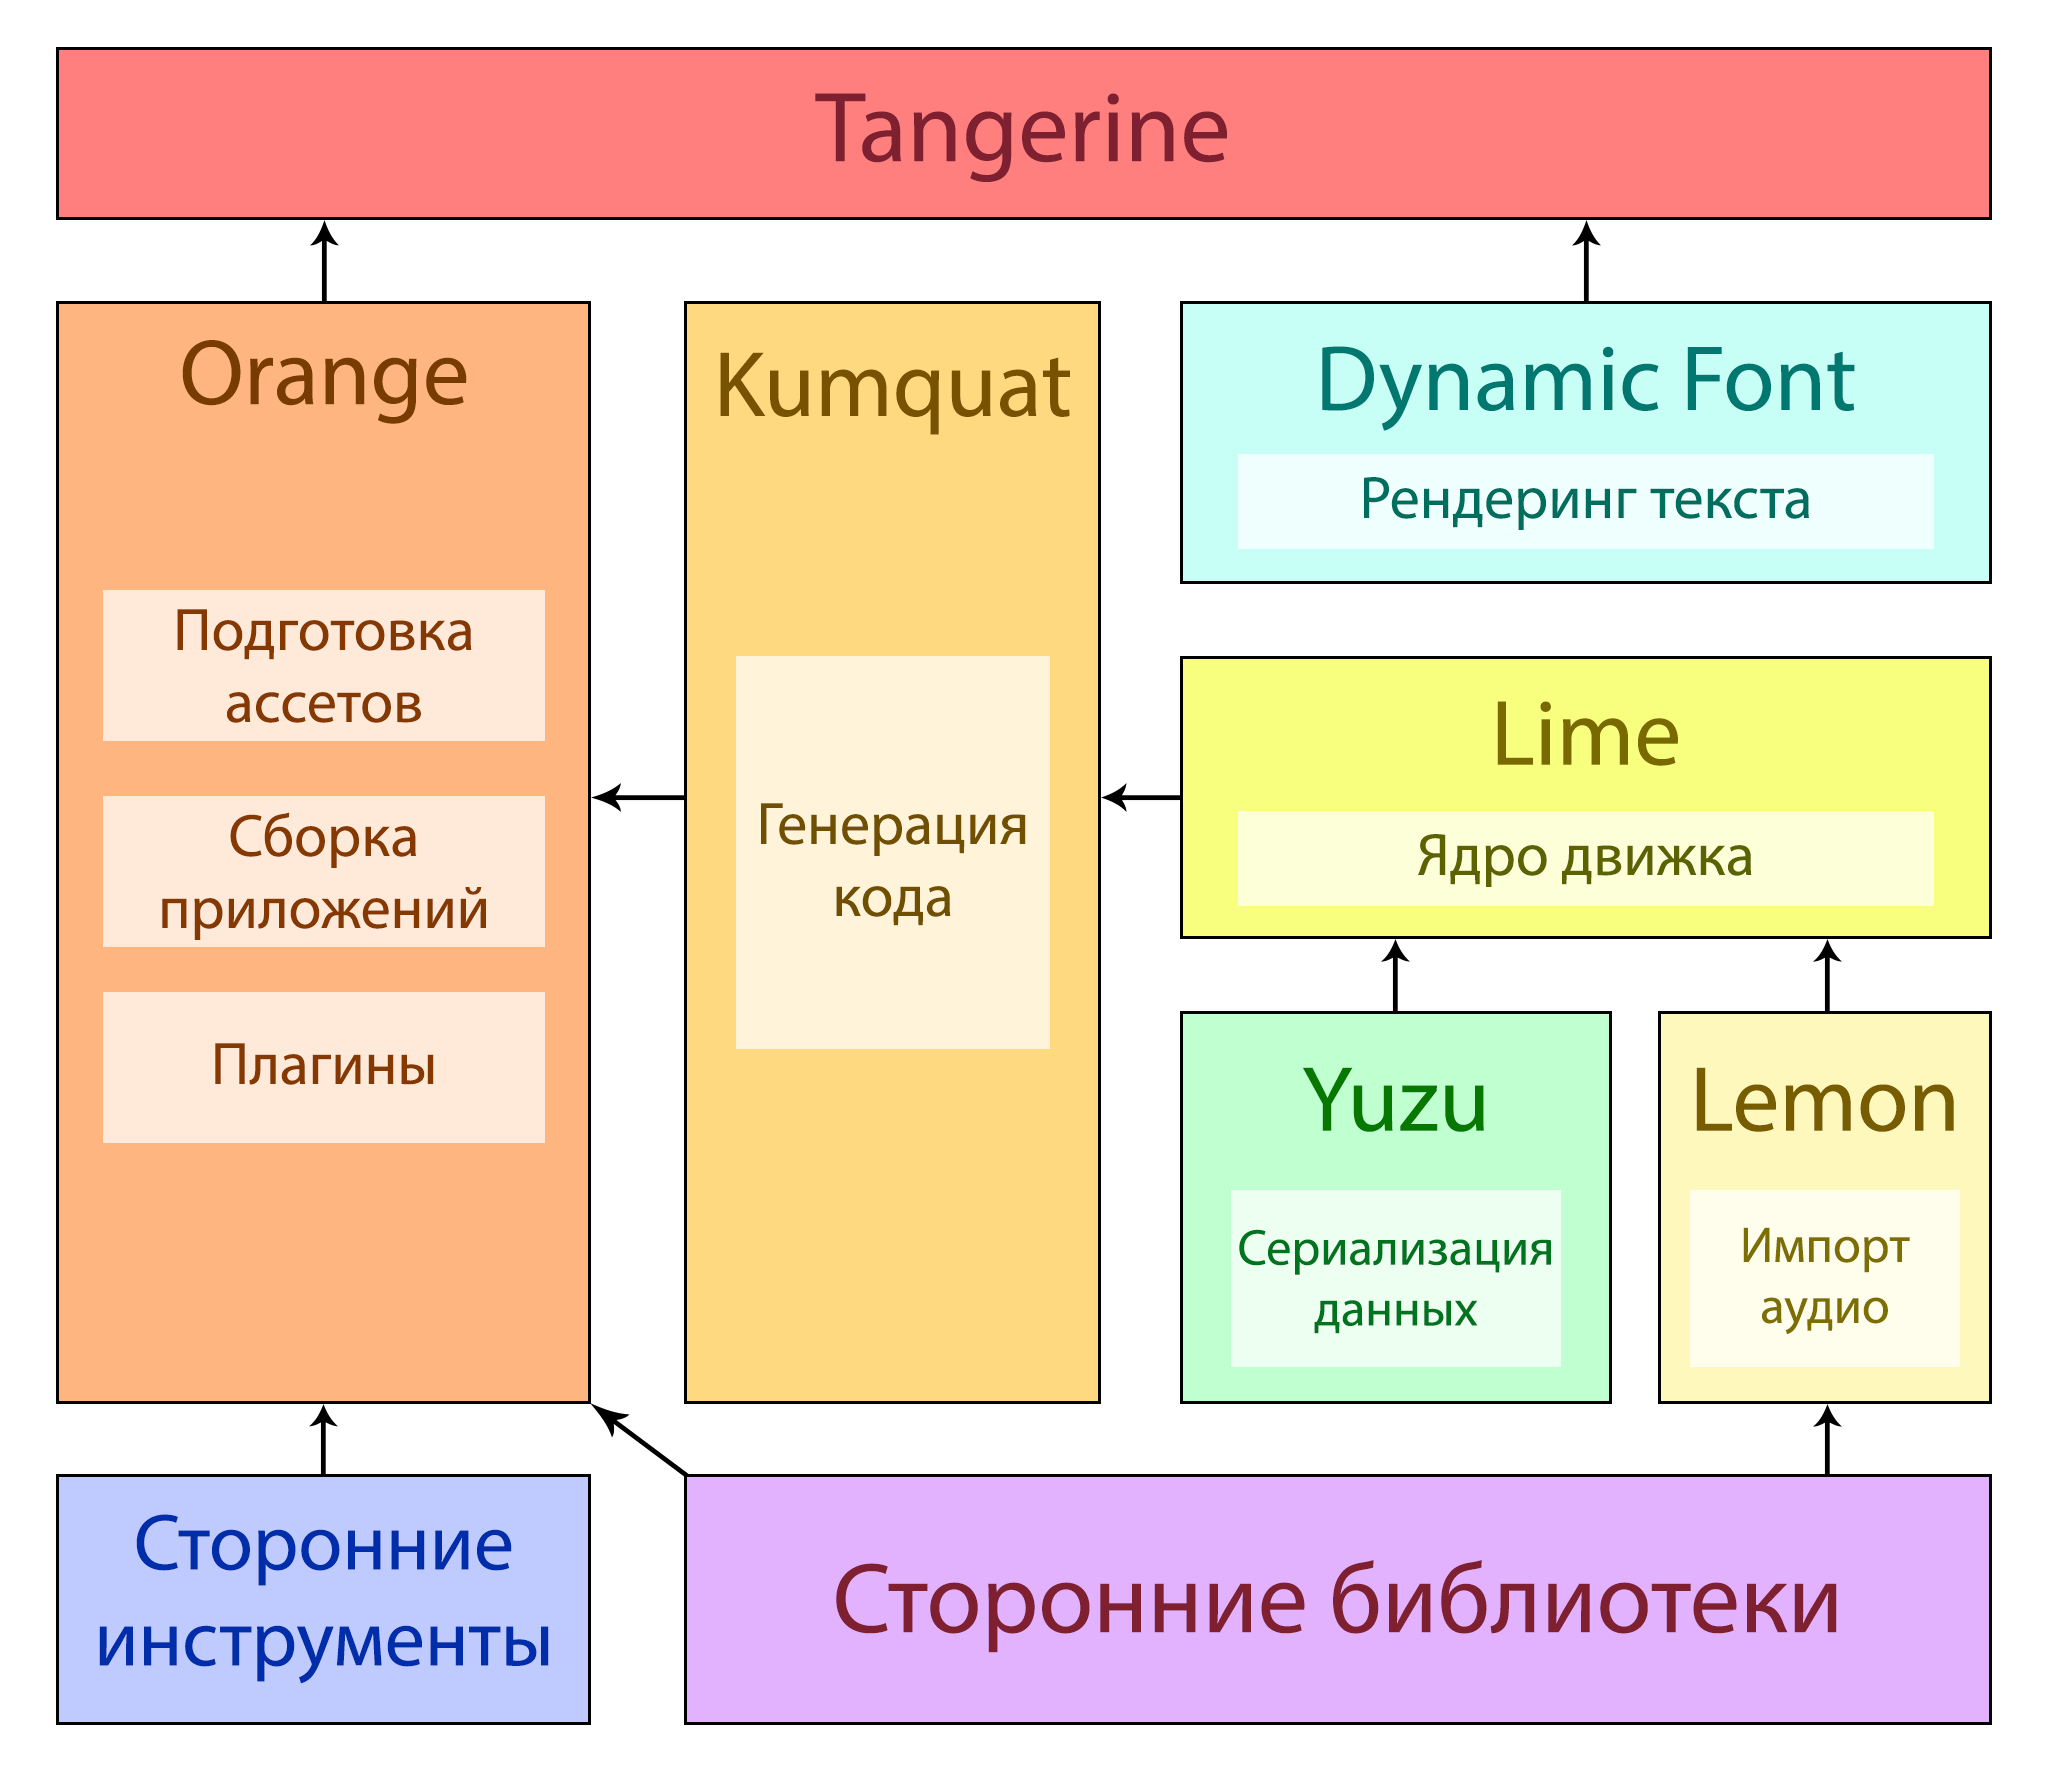
\includegraphics[width=1\linewidth]{images/CitrusScheme.png}
					\caption{Схема модулей движка Citrus}
					\label{img:CitrusScheme}
				\end{figure}
			\subsubsection{Текстовый редактор}
				\par Текстовый редактор это компьютерная программа (или её часть), 
				предназначенная для создания и изменения текстовых данных (в том числе 
				текстовых файлов). Часто редакторы предоставляют пользователям дополнительные 
				возможности, такие как: копирование и вставка, поиск и замена текста, 
				форматирование текста (переносы строк, выравнивание и пр.), 
				откат/восстановление изменений \cite{WhatIsATextEditor}. 
				\par Некоторые редакторы, помимо работы с обычным текстом, позволяют также и
				работу со стилизованным текстом (т.н. \textbf{Rich Text}) 
				\cite{DiffBetweenTextFormats}. Так как текстовый формат данных не предполагает
				хранения информации о стиле текста, в редакторах тексты обрамляются в различные
				языки разметки (например, HTML), либо используется внутреннее двоичное 
				представление.
				\par Для успешной работы текстового редактора необходимо, чтобы были
				реализованы три его основные компоненты: \cite{CraftOfTextEditing}
				\begin{enumerate}
					\item Обработка внутреннего представления текста --- текст необходимо
					эффективным образом хранить и изменять, наивный подход к этой части
					редактора приведёт к значительному (в случае работы с большими объемами
					данных -- к фатальному) падению производительности всего редактора.
					\item Отрисовка --- текст необходимо правильно отрисовать с учетом размеров
					окна и применённых стилей (шрифт, выравнивание, переносы слов).
					\item Обработка пользовательского ввода --- приём команд
					(вставка, удаление элемента, перевод курсора и~пр.) и передача их
					обработчику внутреннего представления.
				\end{enumerate}
			\subsubsection{Обработка текста в Citrus}
				\par Представление текстовых данных и работа с ними -- важная часть игрового
				движка, поскольку значительная часть важной игровой информации сообщается 
				пользователю в текстовом виде. \textbf{Вставить инфу о классах, занимающихся
				текстом (IText, RichText, SimpleText, TextParser, TextStyle, TextRenderer,
				Editor)} 
				В Citrus есть классы, обеспечивающие обработку ввода и отрисовку текста, 
				однако они реализованы неэффективно, что выражается в резком падении 
				производительности с увеличением длины текста. Это приводит к увеличению
				требований к процессору для поддержания высокой частоты кадров. При дальнейшем
				увеличении объема текста работа программ сильно замедляется, что критично для
				игровых проектов, и составляет значительные неудобства при работе со средствами
				визуального редактирования в движке. Также стоит отметить, что несмотря на
				возможность корректно отображать многострочный текст, текущая система слабо
				приспособлена для его редактирования.
				\par В данный момент эти проблемы решаются обходным путём, т.е. число
				использований многострочного редактора сведено к минимуму, а появления больших
				объемов текста стараются, по возможности, не допускать. В игровых проектах
				число больших текстов невелико, а во время работы с визуальной частью движка
				неэффективность работы текстовой системы, хоть и замедляет работу, не является
				критическим препятствием.
				\par Для решения данных проблем можно переписать всю систему работы с текстом с
				нуля, а можно лишь оптимизировать малоэффективные части. Поскольку разработка 
				подобной системы связана со значительными трудностями, в то время как на уже
				существующую систему опираются многие игровые проекты, я решил лишь внести 
				необходимые изменения в существующую структуру работы.
				\par Первую часть системы -- обработку внутреннего представления текста -- 
				можно использовать как самостоятельную единицу в любых других проектах. Все 
				прочие части завязаны на существующую архитектуру движка Citrus и без него 
				неприменимы.
		\subsection{Неформальная постановка задачи}
			В рамках данной работы требуется выполнить следующие задачи:
			\begin{enumerate}
				\item Изучить имеющиеся подходы к реализации текстовых редакторов
				\item Создать редактор, поддерживающий:
				\begin{itemize}
					\setlength{\itemindent}{-3em}
					\item Просмотр и редактирование обычного (не стилизованного) текста
					\item Эффективную работу с многострочными текстовыми файлами
					\item Эффективную прокрутку текста по вертикали и горизонтали
				\end{itemize}
				\item Сравнить производительность предыдущей версии редактора и этой
				реализации.
			\end{enumerate}
		\subsection{План работ}
			\begin{itemize}
				\item Изучение подходов к реализации текстовых редакторов (1-2 недели)
				\item Изучение кодовой базы движка Citrus в целях нахождения места для внесения
				изменений (1 неделя)
				\item Реализация текстового редактора (4 недели)
				\item Подготовка отчёта (1 неделя)
			\end{itemize}
	\section{Обзор существующих методов решения}
		\subsection{Внутреннее представление текста}
			\par Для хранения и обработки текстовых данных используются различные подходы,
				хотя общее число зарекомендовавших себя относительно невелико.
				\cite{TextEditorDataStructures}.
			\par Для работы текстового редактора любая из структуру должна поддерживать, как 
			минимум, следующие операции: вставку и удаление символов, получение элемента по его
			номеру, получение элемента по строке и столбцу.
			\subsubsection{Массив символов}
				\par Наиболее очевидный способ хранения текста. Вся текстовая информация
				располагается в одном массиве. Это накладывает большие ограничения на скорость
				удаления и вставки \cite{StringsReference}. 
				\par Для удаления необходимо сдвинуть все элементы массива, начиная с позиции
				последнего удаляемого элемента, влево на число позиций, равное размеру
				удаляемой последовательности. Для вставки нужно сдвинуть все элементы, начиная
				с позиции вставки, вправо на число позиций, равное размеру удаляемой
				последовательности, а затем вставить последовательность в позицию вставки.
				\par Алгоритмическая сложность удаления и вставки -- $O(n)$. Учитывая 
				количество символов, зачастую присутствующее в тексте, это чудовищно плохой 
				показатель.
				\par Сложность получения элемента по номеру -- $O(1)$, поскольку достаточно
				применить адресную арифметику. В то же время, сложность получения элемента по
				строке и столбцу -- $O(n)$, потому что необходимо пробежаться по всем элементам
				массива, подсчитывая количество строк, до момента достижения необходимой
				позиции.
				\par Несмотря на недостаточную эффективность, у подхода есть одно преимущество
				-- его очень легко реализовать. Однако для реализации чего-либо кроме
				простейшего однострочного поля ввода стоит предпочесть другие варианты.
			\subsubsection{Буферное окно (Gap buffer)}
				\par Текст хранится в массиве, однако часть строки не заполнена и служит для
				заполнения в случае необходимости вставки элемента. Так как в текстовых
				редакторах изменения, зачастую, происходят около одного места (позиция 
				курсора), то операции вставки и удаления можно выполнять очень быстро.
				Узким местом подхода является тот факт, что при интенсивных вставках элементов
				буфер может закончиться, в этом случае его необходимо будет расширить заново,
				выполнив операцию сдвига всех элементов вправо с определенной позиции на размер
				буфера. Перемещение буфера к позиции курсора так же требует времени, в худшем 
				случае (курсор переместили от начала текста к его концу) необходимо сдвинуть
				все элементы в массиве \cite{GapBufferArticle}.
				\par Факт эффективности подхода основан на предположении, что стоимость
				перемещения курсора и расширения буфера амортизируется с помощью прочих,
				дешевых операций, поскольку операции перемещения курсора и расширения буфера
				довольно редки по сравнению с операциями вставки.
				\par Алгоритмическая сложность удаления и вставки, в худшем случае, $O(n)$. Для
				данного подхода затруднительно оценить среднестатистическую сложность.
				\par Сложность получения элемента по индексу, как и в случае с обычным 
				массивом, $O(1)$, адресная арифметика всё так же применима при условии, что
				текущий размер буфера всегда известен. Сложность получения элемента по строке и
				столбцу, по тем же причинам, что и у обычного массива, составляет $O(n)$.
				\par Данный подход легко реализуем и даёт значительный прирост
				производительности по сравнению с использованием обычного массива, однако он не
				рассчитан на работу с большими файлами, поскольку в них стоимость операций 
				перемещения курсора и расширения буфера чрезвычайно высоки.
				\par Тем не менее, данный подход нашел применение во многих текстовых
				редакторах, в том числе в весьма известных (например, Emacs
				\cite{EmacsGapBuffer}).
				\par Пример работы. Исходное состояние:
				$$Lorem~ipsum~dolor~sit~[~~~~~~~~~~~~]~adipiscing.$$
				\par Пользователь добавляет текст:
				$$Lorem~ipsum~dolor~sit~amet,[~~]~adipiscing.$$
				\par Пользователь перемещает курсор
				$$Lorem~ipsum~dolor~sit~[~~]~amet,~adipiscing.$$
				\par Пользователь добавляет текст, полностью заполняющий буфер. Система
				расширяет буфер:
				$$Lorem~ipsum~dolor~sit~consectetur[~~~~~~~~~~]~amet,~adipiscing.$$
			\subsubsection{Связный список}
				\par Элементы (например, символы) хранятся в узлах односвязного списка. При 
				таком подходе операции вставки и удаления выполняются очень быстро, поскольку 
				сводятся к манипуляциям с указателями. Проблемой в данном случае становится 
				операция получения элемента по некоторому индексу, поскольку необходимо пройти 
				по указателям от начала и до требуемого элемента, что в худшем случае занимает 
				$O(n)$ времени (для получения элемента по номерам строки и столбца сложность та
				же). Помимо прочего, на хранение большого числа узлов требуется колоссальный 
				объем памяти, поскольку в одном узле хранится лишь по одному символу
				\cite{LinkedListReference}. 
				\par Преимуществом этого подхода является тот факт, что в узлах, помимо
				информации о символе, можно хранить и прочую информацию, например, информацию
				о стиле текста.
			\subsubsection{Набор строк}
				\par Предыдущие варианты реализации текстовых редакторов не ориентированы на
				применение в многострочных редакторах. Использование набора строк --
				естественное решение этой проблемы. Текст представляется в виде набора
				массивов, каждый из которых хранит только по одной строке текста. Стоит
				отметить, что вместо обычных массивов можно использовать описанные выше
				подходы для увеличения эффективности. Использование набора строк позволяет
				оптимизировать отрисовку. Зная номера строк, в данный момент помещающихся в 
				активное окно, можно быстро к ним обратиться и отрисовать только строго
				необходимый объем текста. 
				\par Этот подход раскрывается при использовании в многострочных редакторах,
				поскольку позволяет за $O(1)$ обращаться к элементам по номерам строки и
				столбца.
			\subsubsection{Верёвка (Rope)}
				\par \textbf{Потом вставить}

			\subsubsection{Таблица кусочков (Piece Table)}
				\par Эффективная структура данных, используемая во многих современных 
				текстовых редакторах \cite{PieceTableArticle}. Используется несколько потоков
				(файлов) -- исходный и добавочный. Исходный поток используется только для 
				чтения. В добавочный данные добавляются и читаются из него, но не удаляются.
				Вместо хранения самих символов, в структуре хранится информация о текстовых 
				фрагментах, а именно: позиция начала фрагмента в потоке (файле), его длина, 
				исходный ли это поток или добавочный. При добавлении новых символов они
				записываются в добавочный поток, а в таблицу заносится новый фрагмент. При
				вставке текста, в случае если позиция нового фрагмента содержится внутри
				существующего, возможно разбиение фрагментов на две части, тогда в левой части
				фрагмента остаётся информация о части текста, лежащей до нового фрагмента, а в 
				правой -- после. Во время удаления от фрагментов "отрезаются" части, либо весь
				фрагмент удаляется целиком.
				\par Таблица кусочков это лишь структура данных для хранения информации о
				тексте, настоящую эффективность данному подходу придаёт способ хранения
				кусочков. Одним из наиболее эффективных способов является использование 
				расширяющегося дерева (Splay Tree). Это сбалансированное бинарное дерево 
				поиска, в котором элементы, к которым в последний раз было произведено
				обращение, перемещаются в корень. Это свойство особенно эффективно при
				использовании в текстовых редакторах, поскольку в них большая часть изменений
				производится около одного места -- позиции курсора \cite{SplayTreeArticle}.
				\par При использовании расширяющегося дерева сложность вставки и удаления
				составляет $O(log~m)$, где $m$ -- число фрагментов в дереве. Операция получения
				элемента так же выполняется за $O(log~m)$, однако стоит учесть, что
				требуются дополнительные затраты времени на чтение данных из потока.
				\par Операция получения элемента по номерам строки и столбца в случае наивной
				реализации имеет сложность $O(n)$, где $n$ -- число символов в тексте, однако
				зачастую применяются различные техники для оптимизации этой операции.
				\par Все вышеперечисленные сложности описаны для худшего случая, в случае
				работы с текстом в позиции курсора операции будут выполнены значительно 
				быстрее, поскольку все необходимые элементы будут находиться близко к корню
				дерева, благодаря чему для достижения нужной позиции не потребуется совершать
				полный пробег по дереву.
				\textbf{Вставить картинку}

		%\begin{center}
		%	\begin{tabular}{ |l|c|r|}
		%		\hline
		%		a & b & c \\
		%		\hline
		%	\end{tabular}
		%\end{center}
		\par \textbf{Вывод}
	\section{Требования к окружению}
		\subsection{Требования к аппаратному обеспечению}
			\par Поскольку текстовый редактор является частью движка Citrus и не существует 
			без него, то ниже приведены общие требования для запуска движка и игровых проектов,
			сделанных на его основе.
			\begin{itemize}
				\item GPU с поддержкой OpenGL
				\item CPU Apple A6  или лучше
				\item \textbf{Что-то еще? Уточнить у знатоков}
			\end{itemize}
		\subsection{Требования к программному обеспечению}
			\par Поскольку текстовый редактор является частью движка Citrus и не существует 
			без него, то ниже приведены общие требования для запуска движка и игровых проектов,
			сделанных на его основе.
			\begin{itemize}
				\item ОС Windows 8.1 или выше; MacOS 10 \textbf{Уточнить minor} или выше; дистрибутивы 
				Linux, поддерживающие среду Mono; Android 5 или выше; iOS 10.3.3 или выше
			\end{itemize}
			\textbf{Про дотнет надо, остальное здесь нет.}
	\section{Архитектура системы}
		\par \textbf{Сюда можно перенести кусок цитруса, ответственный за текст}
	\section{Спецификация данных}
		\subsection{Описание формата или структуры данных}
			\textbf{Про тэги не пишу (пока), пишу что потенциально будет вот так}
	\section{Функциональные требования}
		\par\textbf{Пишем про необходимость рисовать многострочный текст, эффективно хранить
		и обновлять, быстро прокручивать, обрабатывать стандартные команды пользовательского
		ввода, ВСЁ АПИ ПОДРОБНО }
		\subsection{Библиотека подпрограмм(классов)}
			\textbf{А тут что?}
	\section{Требования к интерфейсу}
		\textbf{Должна быть возможность скроллить, шрифты, ричтекст (но у меня его нет), кернинг
		С точки зрения UI стоит написать про Editor и CommonText, а именно про 
		шрифты, поддержку переносов, переносы слов и всё такое. С точки зрения API надо писать
		про вещи в духе "Вставить текст" или "Отменить выделение". А нужно ли писать про API?
		Еще можно писать про то, что это всё в окнах, что можно пользоваться тачпадом или 
		клавиатурой (правда именно сам приём команд это не моя проблема), селекшены и прочее 
		для разных устройств}
	\section{Прочие требования}
		\subsection{Требования к надежности}
			\par В случае возникновения ошибок, возможны падения приложений у игроков. Это 
			отрицательным образом сказывается на их вовлеченности в игровой процесс, что
			приводит к падению экономических показателей.
			\par Для предотвращения подобных ситуаций стоит провести тщательное тестирование
			программного кода на предмет ошибок (на низком уровне -- с помощью 
			юнит-тестирования, на высоком -- силами штатных тестировщиков).
		\subsection{Требования к безопасности}
			\textbf{Опускаем раздел или пишем про текстовые поля для ввода паролей}
		\subsection{Требования к производительности}
			Вся цепочка операций (от обработки изменений текста до 
			отрисовки) должна выполняться не более чем за 30 миллисекунд (для отрисовки 30 
			кадров в секунду).
	\section{Проект}
		\subsection{Средства реализации}
			Все части системы были реализованы на языке C\# 7.0, 
			версия .NET Framework 4.7.1, поскольку это стандарт для компании Game Forest.
		\subsection{Структуры данных}
			\textbf{Рассказать про PieceTree только конкретно про мою реализацию, нарисовать 
			схемы. Написать про массивы Words, FittedWords, Lines}
		\subsection{Модули и алгоритмы}
		\par Система состоит из следующих модулей: \textbf{Нужно ли писать про классы, которые я почти не 
		трогал (например, про Renderer и TextParser)?}:
		\begin{itemize}
			\item PieceTree --- структура данных \textbf{Вообще-то класс} для обработки 
			внутреннего представления текста
			\item SubEditor --- класс, обеспечивающий доступ к PieceTree и служащий для 
			обработки вызовов высокого уровня \textbf{Это так пишется?} (например, 
			"Переместить курсор", "Вставить символ")
			\item TextParser --- класс, назначение которого - выделить набор фрагментов -- 
			слов, пробелов, переносов строки -- из исходного текста
			\item TextRenderer --- класс, в котором слова разделяются по строкам с учетом 
			максимальных размеров виджета, а затем каждой строки вычисляется её позиция 
			в пикселях
			\item Renderer --- класс, выполняющий отрисовку текста
			\item CommonText --- связующее звено между модулями
			\item Editor --- класс, обеспечивающий обработку пользовательского ввода (и 
			передачу соответствующих команд низкоуровневым модулям)
		\end{itemize}
		\textbf{Ну и пишем дальше, подбавляем подробностей. Алгоритмов у меня, кажется, нет.}
		\subsection{Проблемы и решения}
			\par В ходе разработки пришлось столкнуться со следующими \textbf{дописать 
			подводку}
			\begin{itemize}
				\item Предыдущий код TextRenderer трудно читается из-за функций размером в
				200 строк. Рефакторинг значительно улучшил читаемость \textbf{А мои функции 
				усложнили ха-ха}
				\item \textbf{Что-то там еще было}
			\end{itemize}
		\subsection{Стандарт кодирования}
			\textbf{Пишем стандарт Game Forest}
		\subsection{Проект интерфейса}
			\textbf{Кажется, мне это не особо нужно, но для примера можно вставить скрины
			CommonText, ScrollView и Editor}
	\section{Реализация и тестирование}
		\textbf{Всё по плану}
		\textbf{Родить акт о внедрении}
		\subsection{Вычислительный эксперимент}
			\textbf{Тут вставить обещанное исследование/сравнение производительности}
	\section*{Заключение}
		\textbf{Всё по плану}
	\newpage
	\bibliographystyle{ugost2008ls}
	\bibliography{references}
	
\end{document}